\chapter{Block Pointers and Indirect Blocks}\label{chap:blkptr}

Data is transferred between disk and main memory in units called blocks.
A block pointer \lstinline{blkptr_t} is a 128 byte ZFS structure used
to physically locate, verify, and describe blocks of data on disk.
The 128 byte \lstinline{blkptr_t} structure layout is shown in the
Figure~\ref{fig:blkptr}.

\begin{figure}[ht!]
  \centering
  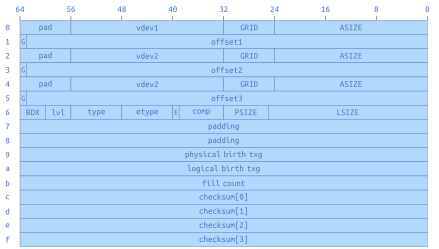
\includegraphics[width=\textwidth]{Figures/zfs_blkptr.pdf}
  \caption{Block pointer structure showing byte by byte usage}
  \label{fig:blkptr}
\end{figure}

Normally,
block pointers point (via their DVAs) to a block which holds data.
If the data that we need to store is very small,
this is an inefficient use of space,
Additionally, reading these small blocks tends to generate
more random reads.
Embedded-data Block Pointers was introduced.
It allows small pieces of data
(the "payload", upto 112 bytes) embedded in the block pointer,
the block pointer doesn't point to anything then.
The layout of an embedded block pointer is as Figure~\ref{fig:embedded}.

\begin{figure}[ht]
  \centering
  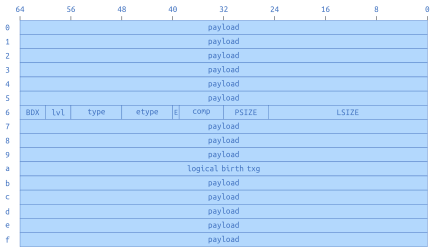
\includegraphics[width=\textwidth]{Figures/zfs_embedded_blkptr.pdf}
  \caption{Embedded Block Pointer Layout}
  \label{fig:embedded}
\end{figure}

\section{Data Virtual Address}

The \emph{data virtual address}, or \emph{DVA} is the name
given to the combination of the vdev and offset portions of the block pointer,
for example the combination of vdev1 and offset1 make up a DVA (dva1).
ZFS provides the capability of storing up to three copies of the data pointed to by the block pointer,
each pointed to by a unique DVA (dva1, dva2, or dva3).
The data stored in each of these copies is identical.
The number of DVAs used per block pointer is purely a policy decision
and is called the “wideness” of the block pointer:
single wide block pointer (1 DVA),
double wide block pointer (2 DVAs),
and triple wide block pointer (3 DVAs).

The \emph{vdev} portion of each DVA is a 32 bit integer
which uniquely identifies the vdev ID containing this block.
The offset portion of the DVA is a 63 bit integer value
holding the offset (starting after the vdev labels (L0 and L1) and boot block)
within that device where the data lives.
Together,
the vdev and offset uniquely identify the block address of the data it points to.

The value stored in offset is the offset in terms of sectors (512 byte blocks).
To find the physical block byte offset from the beginning of a slice,
the value inside offset must be shifted over ($\ll$) by $9$ ($2^9 =512$)
and this value must be added to \verb|0x400000|
(size of two vdev\_labels and boot block).
\[
physical\ block\ address = (\mathit{offset} \ll 9) + 0x400000~(4MB)
\]

\section{GRID}

Raid-Z layout information, reserved for future use.

\section{Gang}

A \emph{gang block} is a block whose contents contain block pointers.
Gang blocks are used when the amount of space requested is not available in a contiguous block.
In a situation of this kind,
several smaller blocks will be allocated
(totaling up to the size requested)
and a gang block will be created to contain the block pointers for the allocated blocks.
A pointer to this gang block is returned to the requester,
giving the requester the perception of a single block.

Gang blocks are identified by the ``G'' bit.

\begin{table}[ht]
  \caption{Gang Block Values}
  \label{tbl:gang_block}
  \centering
  \begin{tabular}{ll}
    \toprule
    \textbf{``G'' bit value} &     \textbf{Description}\\
    \midrule
    0 & non-gang block\\
    1 & gang block\\
    \bottomrule
  \end{tabular}
\end{table}

Gang blocks are 512 byte sized,
self checksumming blocks.
A gang block contains up to 3 block pointers
followed by a 32 byte checksum.
The format of the gang block is described by the following structures.

\begin{lstlisting}[style=c]
typedef struct zio_gbh {
        blkptr_t		zg_blkptr[SPA_GBH_NBLKPTRS];
        uint64_t		zg_filler[SPA_GBH_FILLER];
        zio_eck_t		zg_tail;
} zio_gbh_phys_t;
\end{lstlisting}

\begin{description}
  \item[zg\_blkptr]
    Array of block pointers. Each 512 byte gang block can hold up to 3 block pointers.

  \item[zg\_filler]
    The filler fields pads out the gang block so that it is nicely byte aligned.
\begin{lstlisting}[style=c]
typedef struct zio_eck {
        uint64_t	zec_magic;
        zio_cksum_t	zec_cksum;
} zio_eck_t;
\end{lstlisting}

  \item[zec\_magic]
    ZIO block tail magic number.
    The value is \verb|0x210da7ab10c7a11| (zio-data-bloc-tail).
\begin{lstlisting}[style=c]
typedef struct zio_cksum {
        uint64_t	zc_word[4];
} zio_cksum_t;
\end{lstlisting}

  \item [zc\_word]
      Four 8 byte words containing the checksum for this gang block.
\end{description}

\section{Checksum}

By default ZFS checksums all of its data and metadata.
ZFS supports several algorithms for checksumming including fletcher2, fletcher4,
and SHA-256 (256-bit Secure Hash Algorithm in FIPS 180-2,
available at \href{http://csrc.nist.gov/cryptval}{http://csrc.nist.gov/cryptval}).
The algorithm used to checksum this block
is identified by the 8 bit integer stored in the cksum portion of the block pointer. The
following table pairs each integer with a description and algorithm
used to checksum this block's contents.

A 256 bit checksum of the data is computed for each block
using the algorithm identified in cksum.
If the cksum value is 2 (off),
a checksum will not be computed
and checksum[0], checksum[1], checksum[2], and checksum[3] will be zero.
Otherwise,
the 256 bit checksum computed for this block is stored
in the checksum[0], checksum[1], checksum[2], and checksum[3] fields.

\emph{
Note:
The computed checksum is always of the data,
even if this is a gang block.
Gang blocks (see above) and zilog blocks (see Chapter~\ref{chap:zil}) are self checksumming.
}

\begin{LongTable3Columns}{Name}{Value}{Algorithm}{Checksum Values and associated algorithms}{chksum_values}{lll}
  {
    on  & 1 & fletcher2\\
    off & 2 & none\\
    label & 3 & SHA-256\\
    gang header & 4 & SHA-256\\
    zilog & 5 & fletcher2\\
    fletcher2 & 6 & fletcher2\\
    fletcher4 & 7 & fletcher4\\
    SHA-256 & 8 & SHA-256\\
    zilog2 & 9 & fletcher2\\
    noparity & 10 & \textcolor{red}{???}\\
    SHA-512 & 11 & SHA-512\\
    skein & 12 & \textcolor{red}{???}\\
  }
\end{LongTable3Columns}

\section{Compression}

ZFS supports several algorithms for compression.
The type of compression used to compress this block is stored
in the comp portion of the block pointer.

\begin{LongTable3Columns}{Description}{Value}{Algorithm}{Compression Values and associated algorithms}{comp_values}{lll}
  {
    on & 1 & lz4\\
    off & 2 & none\\
    lzjb & 3 & lzjb\\
    empty & 4 & empty\\
    gzip level 1$\sim$9 & 5$\sim$13 & gzip1$\sim$9\\
    zle & 14 & zle\\
    lz4 & 15 & lz4\\
    zstd & 16 & zstd\\
  }
\end{LongTable3Columns}

\section{Block Size}

The size of a block is described by three different fields in the block pointer;
\emph{psize}, \emph{lsize}, and \emph{asize}.

\begin{description}
\item[lsize]
  Logical size. The size of the data without compression, raidz or gang overhead.

\item[psize]
  Physical size of the block on disk after compression.

\item[asize]
  Allocated size,
  total size of all blocks allocated to hold this data
  including any gang headers or Raid-Z parity information
\end{description}

If compression is turned off and ZFS is not on Raid-Z storage,
lsize, asize, and psize will all be equal.

All sizes are stored as the number of 512 byte sectors (minus one)
needed to represent the size of this block.

\section{Endian}

ZFS is an adaptive-endian filesystem
(providing the restrictions described in Chapter~\ref{chap:vdev})
that allows for moving pools across machines with different architectures:
little endian vs. big endian.
The “E” portion of the block pointer indicates
which format this block has been written out in.
Block are always written out in the machine's native endian format.

\begin{table}[ht]
  \caption{Endian Values}
  \label{tbl:endian_values}
  \centering
  \begin{tabular}{ll}
    \toprule
    \textbf{Endian} &     \textbf{Value}\\
    \midrule
    Little Endian & 1\\
    Big Endian & 2\\
    \bottomrule
  \end{tabular}
\end{table}

If a pool is moved to a machine with a different endian format,
the contents of the block are byte swapped on read.

\section{Type}

The \emph{type} portion of the block pointer indicates what type of data this block holds.
The type can be the following values.
More detail is provided in Chapter~\ref{chap:dmu} regarding object types.

\begin{LongTable2Columns}{Type}{Value}{Object Types}{obj_types}{lr}
  {
   DMU\_OT\_NONE & 0\\
   DMU\_OT\_OBJECT\_DIRECTORY & 1\\
   DMU\_OT\_OBJECT\_ARRAY & 2\\
   DMU\_OT\_PACKED\_NVLIST & 3\\
   DMU\_OT\_NVLIST\_SIZE & 4\\
   DMU\_OT\_BPLIST & 5\\
   DMU\_OT\_BPLIST\_HDR & 6\\
   DMU\_OT\_SPACE\_MAP\_HEADER & 7\\
   DMU\_OT\_SPACE\_MAP & 8\\
   DMU\_OT\_INTENT\_LOG & 9\\
   DMU\_OT\_DNODE & 10\\
   DMU\_OT\_OBJSET & 11\\
   DMU\_OT\_DSL\_DATASET & 12\\
   DMU\_OT\_DSL\_DATASET\_CHILD\_MAP & 13\\
   DMU\_OT\_OBJSET\_SNAP\_MAP & 14\\
   DMU\_OT\_DSL\_PROPS & 15\\
   DMU\_OT\_DSL\_OBJSET & 16\\
   DMU\_OT\_ZNODE & 17\\
   DMU\_OT\_ACL & 18\\
   DMU\_OT\_PLAIN\_FILE\_CONTENTS & 19\\
   DMU\_OT\_DIRECTORY\_CONTENTS & 20\\
   DMU\_OT\_MASTER\_NODE & 21\\
   DMU\_OT\_DELETE\_QUEUE & 22\\
   DMU\_OT\_ZVOL & 23\\
   DMU\_OT\_ZVOL\_PROP & 24\\
  }
\end{LongTable2Columns}

\section{Level}

The \emph{level} portion of the block pointer is the number of levels
(number of block pointers
which need to be traversed to arrive at this data.)
See Chapter~\ref{chap:dmu} for a more complete definition of level.

\section{Fill}

The \emph{fill} count describes the number of non-zero block pointers under this block pointer.
The fill count for a data block pointer is 1,
as it does not have any block pointers beneath it.
The fill count is used slightly differently for block pointers of type \lstinline{DMU_OT_DNODE}.
For block pointers of this type,
the fill count contains the number of free dnodes beneath this block pointer.
For more information on dnodes see Chapter~\ref{chap:dmu}.

\section{Birth Transaction}

The \emph{birth transaction} stored in the
``physical birth txg'' and ``logical birth txg''
block pointer field is a 64 bit integer
containing the transaction group number
in which this block pointer was allocated.

\section{Padding}

The two padding fields in the block pointer are space reserved for future use.
